\documentclass[review,onefignum,onetabnum]{siamart190516}
%\usepackage{natbib}
%\usepackage[sort]{cite}
\pdfoutput=1
%\usepackage[colorlinks=true,urlcolor=blue,citecolor=blue,linkcolor=blue]{hyperref}
\usepackage[english]{babel}
\usepackage[utf8]{inputenc}
\usepackage[T1]{fontenc}
\usepackage{amssymb}
\usepackage{tabularx}
\usepackage{quoting}
\usepackage{upquote}
\usepackage{subcaption}
\usepackage{multicol}
\usepackage[framemethod=TikZ]{mdframed}
\usetikzlibrary{shapes}
\usetikzlibrary{snakes}
\usepackage{wrapfig}
%\usepackage{caption}
%\usepackage[plain]{algorithmic}
\usepackage[linesnumbered, ruled, vlined, algo2e]{algorithm2e}
\usepackage{algpseudocode}
\usepackage{rotating}
%\usepackage{cite}
\usepackage{booktabs}
%\usepackage{unicode-math}
%\usepackage{algorithm}% http://ctan.org/pkg/algorithm
%\usepackage{algpseudocode}% http://ctan.org/pkg/algpseudocode
\usepackage{xcolor}% http://ctan.org/pkg/xcolor
\makeatletter
\newsavebox{\@brx}
\newcommand{\llangle}[1][]{\savebox{\@brx}{\(\m@th{#1\langle}\)}%
  \mathopen{\copy\@brx\kern-0.5\wd\@brx\usebox{\@brx}}}
\newcommand{\rrangle}[1][]{\savebox{\@brx}{\(\m@th{#1\rangle}\)}%
  \mathclose{\copy\@brx\kern-0.5\wd\@brx\usebox{\@brx}}}
\makeatother
\usepackage{bbm}
\usepackage{jlcode}
\usepackage{graphicx}
\usepackage{amsmath,color}
\usepackage{mathrsfs}
\usepackage{float}
\usepackage[normalem]{ulem}
\usepackage{makecell}
\usepackage{indentfirst}
\usepackage{txfonts}
\usepackage[epsilon, tsrm, altpo]{backnaur}

\makeatletter
\def\parsept#1#2#3{%
    \def\nospace##1{\zap@space##1 \@empty}%
    \def\rawparsept(##1,##2){%
        \edef#1{\nospace{##1}}%
        \edef#2{\nospace{##2}}%
    }%
    \expandafter\rawparsept#3%
}
\makeatother
\DeclareMathAlphabet{\mymathbb}{U}{BOONDOX-ds}{m}{n}
\newcommand{\listingcaption}[1]%
{%
\refstepcounter{lstlisting}\hfill%
Listing \thelstlisting: #1\hfill%\hfill%
}%
\newcolumntype{b}{X}
\newcolumntype{s}{>{\hsize=.7\hsize}X}
\usepackage{listings}
\lstset{
    language=Julia,
    basicstyle=\ttfamily\scriptsize,
    numberstyle=\scriptsize,
    % numbers=left,
    backgroundcolor=\color{gray!7},
    %backgroundcolor=\color{white},
    %frame=single,
    xleftmargin=2em,
    tabsize=2,
    rulecolor=\color{black!15},
    %title=\lstname,
    escapeinside={(*}{*)},
    breaklines=true,
    %breakatwhitespace=true,
    %framextopmargin=2pt,
    %framexbottommargin=2pt,
    frame=bt,
    extendedchars=true,
    inputencoding=utf8,
    columns=fullflexible,
    %escapeinside={(*@}{@*)},
}

\tolerance=1
\emergencystretch=\maxdimen
\hyphenpenalty=1000
\hbadness=1000

\makeatletter

%%%%%%%%%%%%%%%%%%%%%%%%%%%%%% User specified LaTeX commands.

%Journal reference.  Comma sets off: name, vol, page, year
\def\journal #1, #2, #3, 1#4#5#6{{\sl #1~}{\bf #2}, #3 (1#4#5#6) }
\def\pr{\journal Phys. Rev., }
\def\prb{\journal Phys. Rev. B, }
\def\prl{\journal Phys. Rev. Lett., }
\def\pl{\journal Phys. Lett., }
%\def\np{\journal Nucl. Phys., }


%%%%%%%%%%%%%%%%%%%%%%%%%%%%%%%%%%%%%%%%%%%%%%%%%%%%%%%%%%%%%%%%%%%%%%%%%%%%%%%%%%%%%%%%%%%%%%%%%%%%%%%%%%%%%%%%%%%%%%%%%%%%%%%%%%%%%%%%%%%%%%%%%%%%%%%%%%%%%%%%%%%%%%%%%%%%%%%%%%%%%%%%%%%%%%%%%%%%%%%%%%%%%%%%%%%%%%%%%%%%%%%%%%%%%%%%%%%%%%%%%%%%%%%%%%%%


%\usepackage{CJK}
%\usepackage[colorlinks, citecolor=blue]{hyperref}
\DeclareMathOperator*{\argmax}{arg\,max}

%%%%%% Shortcut related
\newcommand{\<}{\langle}
\renewcommand{\>}{\rangle}
\newcommand{\out}{{\vx^L}}
\newcommand{\inp}{{\vx^0}}
\newcommand{\cquad}{{{ }_{\quad}}}
\newcommand{\pluseq}{\mathrel{+}=}
\newcommand{\minuseq}{\mathrel{-}=}
\newcommand{\vx}{{\mathbf{x}}}
\newcommand{\vg}{{\mathbf{g}}}
\newcommand{\vp}{{\mathbf{p}}}
\newcommand{\vy}{{\mathbf{y}}}
\newcommand{\Var}{{\mathrm{Var}}}
\newcommand{\Mean}{{\mathrm{E}}}
\newcommand{\vvalue}{{\texttt{value}}}
\newcommand{\grad}{{\texttt{grad}}}
\newcommand{\parameter}{{\texttt{parameter}}}
%%%%%% Convention related
\newcommand{\SWAP}{{\rm SWAP}}
\newcommand{\CNOT}{{\rm CNOT}}
\newcommand{\bigO}{{\mathcal{O}}}
\newcommand{\X}{{\rm X}}
\renewcommand{\H}{{\rm H}}
\newcommand{\Rx}{{\rm Rx}}
\renewcommand{\v}[1]{{\bf #1}}
\newcommand{\dataset}{{\mathcal{D}}}
\newcommand{\wfunc}{{\psi}}
\newcommand{\SU}{{\rm SU}}
\newcommand{\UU}{{\rm U}}
\newcommand{\thetav}{{\boldsymbol{\theta}}}
\newcommand{\gammav}{{\boldsymbol{\gamma}}}
\newcommand{\thetai}{{\theta^\alpha_l}}
\newcommand{\Expect}{{\mathbb{E}}}
\newcommand{\Tr}{{\rm Tr}}
\newcommand{\etc}{{\it etc~}}
\newcommand{\etal}{{\it etal~}}
\newcommand{\xset}{\mathbf{X}}
\newcommand{\fl}{\texttt{fl}}
\newcommand{\pdata}{\mathbf{\pi}}
\newcommand{\q}{\mathbf{q}}
\newcommand{\epdata}{\mathbf{\hat{\pi}}}
\newcommand{\gammaset}{\boldsymbol{\Gamma}}
\newcommand{\ei}{{\mathbf{e}_l^\alpha}}
\newcommand{\vtheta}{{\boldsymbol{\theta}}}
\newcommand{\sigmag}{{\nu}}
\newcommand{\sigmai}[2]{{\sigma^{#2}_{#1}}}
\newcommand{\qi}[1]{{q^{\alpha_{#1}}_{#1}}}
\newcommand{\BAS}{Bars-and-Stripes}
\newcommand{\circled}[1]{\raisebox{.5pt}{\textcircled{\raisebox{-.9pt} {#1}}}}
\newcommand{\qexpect}[1]{{\left\langle #1\right\rangle}}
\newcommand{\expect}[2]{{\mathop{\mathbb{E}}\limits_{\substack{#2}}\left[#1\right]}}
\newcommand{\var}[2]{{\mathop{\mathrm{Var}}\limits_{\substack{#2}}\left(#1\right)}}
\newcommand{\pshift}[1]{{p_{\thetav+#1}}}
\newcommand{\upcite}[1]{\textsuperscript{\cite{#1}}}
\newcommand{\Eq}[1]{Eq.~(\ref{#1})}
\newcommand{\Fig}[1]{Fig.~\ref{#1}}
\newcommand{\Lst}[1]{Listing.~\ref{#1}}
\newcommand{\Tbl}[1]{Table~\ref{#1}}
\newcommand{\Sec}[1]{Sec.~\ref{#1}}
\newcommand{\App}[1]{Appendix~\ref{#1}}
\newcommand{\bra}[1]{\mbox{$\left\langle #1 \right|$}}
\newcommand{\ket}[1]{\mbox{$\left| #1 \right\rangle$}}
\newcommand{\braket}[2]{\mbox{$\left\langle #1 | #2 \right\rangle$}}
\newcommand{\tr}[1]{\mathrm{tr}\mbox{$\left[ #1\right]$}}

\newcommand{\ra}[1]{\renewcommand{\arraystretch}{#1}}

%%%%%% Comment related
\newcommand{\red}[1]{[{\bf  \color{red}{LW: #1}}]}
\newcommand{\xred}[1]{[{\bf  \color{red}{\sout{LW: #1}}}]}
\newcommand{\blue}[1]{[{\bf  \color{blue}{JG: #1}}]}
\newcommand{\violet}[1]{[{\bf  \color{violet}{MLS: #1}}]}
\newcommand{\green}[1]{[{\bf  \color{green}{TZ: #1}}]}
\newcommand{\xgreen}[1]{[{\bf  \color{green}{\sout{TZ: #1}}}]}
\newcommand{\xblue}[1]{[{\bf  \color{blue}{\sout{JG: #1}}}]}
\newcommand{\material}[1]{\iffalse[{\bf  \color{cyan}{Material: #1}}]\fi}
\newcommand{\orange}[1]{\iffalse[{\bf  \color{orange}{Jo: #1}}]\fi}

\newcounter{example}
\newenvironment{example}[1][]{\refstepcounter{example}\par\medskip
   \noindent \textbf{Example~\theexample. #1} \rmfamily}{\medskip}

%\newtheorem{theorem}{\textit{Theorem}}
%\newtheorem{corollary}{\textit Branching Rule}
%\theoremstyle{definition}\newtheorem{definition}{\textit{Definition}}
%\newtheorem{defin}[thm]{Definition}

\makeatother

%\externaldocument{ex_supplement}

\title{Solving the maximum independant set problem by generic programming einsum networks
\thanks{\funding{...}}
}

\author{XXX\thanks{XXX 
  (\email{email}, \url{website}).}
\and YYY\thanks{yyyyy 
  (\email{yyyy}, \email{email}).}
}

\begin{document}

\maketitle

\begin{abstract}
	Solving the maximum independent set size problem by mapping the graph to an einsum network. 
    We show how to obtain the maximum independent set size, the independence polynomial and optimal configurations of a graph by engineering the tensor element algebra.
\end{abstract}

% REQUIRED
\begin{keywords}
  maximum independent set, einsum network
\end{keywords}

% REQUIRED
% 14N07  	Secant varieties, tensor rank, varieties of sums of powers
\begin{AMS}
  05C31, 14N07
\end{AMS}

\section{Introduction}
In this work, we introduce a new method to solve the classic graph problem, finding independent sets.
Given an undirected graph $G = (V,E)$, an independent set $I \subseteq V$ is a set that for any $u,v \in I$, there is no edge connecting $u$ and $v$ in $G$.
Finding the maximum independent set (MIS) size $\alpha(G) \equiv \max_{I}|I|$ belongs to the complexity class NP-complete~\cite{Hastad1996}, which is unlikely to be decided in polynomial time.
It is hard to even approximate this size in polynomial time within a factor $|V|^{1-\epsilon}$ for an arbituary small possitive $\epsilon$.
The naive algorithm of enumerating all configuration space gives a $2^{|V|}$ time solution.
More efficient algorithms to compute the MIS size exactly includes the branching algorithm and dynamic programming.
Without changing the fact of exponential scaling in computing time, the branching algorithm gives a smaller base.
For example, in ~\cite{Xiao2017}, a sophisticated branching algorithm gives a time complexity $1.1893^n n ^{O(1)}$.
The dynamic programming approach~\cite{Courcelle1990,Fomin2013} works better for graphs with small tree width $tw(G)$, it gives an algorithms of complexity $O(2^{tw(G)}tw(G)n)$.
People are interested in solving this problem better not only because it is a NP-complete problem that directly related to other NP-complete prolems like maximal cliques and vertex cover~\cite{Moore2011},
but also for its close relation with physical applications like hard spheres lattice gas model~\cite{Dyre2016}, and Rydberg hamiltonian~\cite{Pichler2018}.
In these applications, knowing the MIS size and one of the optimal solution is not the only goal.
%A set is independent if and only if it is a clique in the graph's complement, so the two concepts are complementary.
%A set is independent if and only if its complement is a vertex cover. Therefore, the sum of the size of the largest independent set $\alpha (G)$ and the size of a minimum vertex cover $\beta (G)$ is equal to the number of vertices in the graph.
People often ask different questions about independent sets in order to understand the landscape of their models better.
These questions includes but not limited to, counting all independent sets, obtaining all indenepent sets of size $\alpha(G)$ and $\alpha(G)-1$,
counting the number of (maximal) independent sets of different sizes.
In this work, we attack this problem by mapping it to an generic ``einsum'' network.
It does not give a better time complexity comparing to dynamic programming, but is versatile enough to answer the above questions by engineering the tensor elements.

\section{Einsum network}
The word ``einsum'' is a shorthand for Einstein's summation, however, modern einsum notation in program is actually invented by a group of programmers.
Einstein's notation is originally proposed as a generalization to of multiplication between two matrices to the contraction between multiple tensors.
Let $A, B$ be two matrices, the matrix multiplication is defined as $C_{ik} = \sum_{j}A_{ij}B_{jk}$.
It is denoted as $C_i^k = A_i^j B_j^k$ in the Einstein's original notation, where the paired subscript and superscript $j$ is a dummy index summed over.
One can map a tensor network to a muti-graph with open edges by viewing a tensor in the expression on the right hand side as a vertex in a graph, a label pairing two tensors as an edge, and the remaining labels as open edges.

\begin{example}
    A tensor networks $C_i^l = A_{ij}^k B^l_k V^j$, where its graphical notation as the following.
One can easily check a label in a tensor network representation appears precisely twice.

\centerline{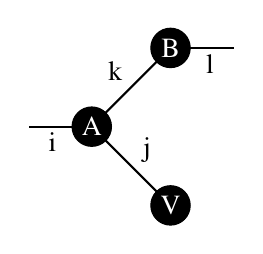
\begin{tikzpicture}
    \def\dx{0};
    \def\r{0.25}
    \def\ax{0}
    \def\ay{0}
    \def\bx{1}
    \def\by{1}
    \def\cx{1}
    \def\cy{-1}
    \filldraw[fill=black] (\ax+\dx,\ax) circle [radius=\r];
    \filldraw[fill=black] (\bx+\dx,\by) circle [radius=\r];
    \filldraw[fill=black] (\cx+\dx,\cy) circle [radius=\r];
    %\draw [black,thick] (\ax+\dx,\ay) .. controls (0.5*\ax+0.5*\bx+\dx+0.2,0.5*\ay+0.5*\by-0.2) .. (\bx+\dx,\by);
    %\draw [black,thick] (\ax+\dx,\ay) .. controls (0.5*\ax+0.5*\bx+\dx-0.2,0.5*\ay+0.5*\by+0.2) .. (\bx+\dx,\by);
    \draw [black,thick] (\ax+\dx,\ay) -- (\bx+\dx,\by);
    \draw [black,thick] (\ax+\dx,\ay) -- (\cx+\dx,\cy);
    \draw [black,thick] (\ax+\dx,\ay) -- (\ax+\dx-0.8,\ay);
    \draw [black,thick] (\bx+\dx,\by) -- (\bx+\dx+0.8,\by);
    \node[color=white] at (\ax+\dx,\ax) {A};
    \node[color=white] at (\bx+\dx,\by) {B};
    \node[color=black] at (0.5*\ax+0.5*\bx-0.2+\dx,0.5*\ay+0.5\by+0.2) {k};
    \node[color=black] at (0.5*\ax+0.5*\cx+\dx+0.2,0.5*\ay+0.5\cy+0.2) {j};
    \node[color=black] at (\ax+\dx-0.5,\ay-0.2) {i};
    \node[color=black] at (\bx+\dx+0.5,\by-0.2) {l};
    \node[color=white] at (\cx+\dx,\cy) {V};
\end{tikzpicture}}

\end{example}

Numpy programmers make a generalization of this notation by not restricting the number of times a label is used by tensors,
hence whether an index appears as a superscript or a subscript makes no sense now.
It has different names in different context, like sum-product network and factor graph~\cite{Bishop2006}.
The graphical representation of an einsum is a hypergraph, where an edge (degree of freedom) can be shared by a arbituary number of nodes (tensors).

\begin{example}
$C_{ijk} = A_{jkm} B_{mil} V_{jm}$ is an einsum but not a tensor network, it represents $C_{ijk} = \sum_{ml}A_{jkm} B_{mia} V_{jm}$.
Its hypergraph representation is as the following, where we use different color to annotate different hyperedges.

\centerline{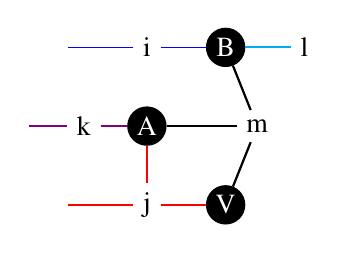
\begin{tikzpicture}[
    dot/.style = {circle, fill, minimum size=#1,
                inner sep=0pt, outer sep=0pt},
    dot/.default = 6pt  % size of the circle diameter 
                    ]  
    \def\dx{0};
    \def\r{0.5cm}
    \def\ax{0}
    \def\ay{0}
    \def\bx{1}
    \def\by{1}
    \def\cx{1}
    \def\cy{-1}
    \node[color=white,fill=black,dot=\r] at (\ax+\dx,\ax) (a) {A};
    \node[color=white,fill=black,dot=\r] at (\bx+\dx,\by) (b) {B};
    \node[color=white,fill=black,dot=\r] at (\cx+\dx,\cy) (v) {V};
    \node at (\ax-0.8,\ay) (k) {k};
    \node at (\bx+0.4,\ay) (m) {m};
    \node at (\ax,\cy) (j) {j};
    \node at (\bx+1,\by) (l) {l};
    \node at (\bx-1,\by) (i) {i};
    \draw[color=blue] (i) -- (b);
    \draw[color=blue] (i) -- (\ax-1,\by);
    \draw[color=cyan,thick] (l) -- (b);
    \draw[color=violet,thick] (k) -- (a);
    \draw[color=violet,thick] (k) -- (\ax-1.5,\ay);
    \draw[color=black,thick] (b) -- (m);
    \draw[color=black,thick] (m) -- (a);
    \draw[color=black,thick] (m) -- (v);
    \draw[color=red,thick] (a) -- (j);
    \draw[color=red,thick] (v) -- (j);
    \draw[color=red,thick] (\ax-1,\cy) -- (j);
\end{tikzpicture}}
\end{example}

In the main text, we stick to the einsum notation rather than the tensor network notation.
As a note to those who are more familiar with tensor network representation,
although one can easily translate an einsum network to the equivalent tensor network by adding $\delta$ tensors (a generalization of identity matrix to higher order).
It can sometime increase the contraction complexity of a graph. We have an example demonstrating this in \App{app:tensorbad}.

\section{Independence polynomial}
One can encode the independent set problem on graph $G$ to an einsum network by placing a rank one tensor of size $2$ on vertex $i$
\begin{equation}
    W(x_i)_{s_i} = \left(\begin{matrix}
        1 \\
        x_i
    \end{matrix}\right)_{s_i},\label{eq:wtensor}
\end{equation}
and a rank two tensor of size $2 \times 2$ on edge $(i,j)$
\begin{equation}
    B_{s_i s_j} = \left(\begin{matrix}
        1  & 1\\
        1 & 0
    \end{matrix}\right)_{s_is_j},\label{eq:btensor}
\end{equation}
where a tensor index $s_i$ is a boolean variable that being 1 if vertex $i$ is in the independent set, 0 otherwise.
It corresponds to a hyperedge in the hypergraph.
$x_i$ is a variable.
The contraction of such an einsum network gives
\begin{equation}
    A(G, \{x_1,\ldots,x_n\}) = \sum\limits_{s_1, s_2, \ldots, s_n = 0}^{1} \prod\limits_{i=1}^n W(x_i)_{s_i} \prod\limits_{(i,j) \in E(G)} B_{s_i s_j}.
\end{equation}
Here, the einsum runs over all vertex configurations $\{s_1,\ldots,s_n\}$ and accumulates the product of tensor elements to the scalar output.
Let $x_i = x$, then the product over vertex tensors gives a factor $x^k$, where $k=\sum_i s_i$ is the vertex set size, 
and the product over edge tensors gives a factor $0$ for configurations not being an independent set.
The contraction of this einsum network gives the independence polynomial~\cite{Ferrin2014, Harvey2017} of $G$
\begin{equation}
I(G, x) = \sum_{k=1}^{\alpha(G)} a_k x^k,
\end{equation}
where $a_k$ is the number of independent sets of size $k$ in $G$, and $\alpha(G)$ is the maximum independent set size.
By mapping the independence polynomial solving problem to the einsum network contraction, one can take the advantage of recently developed techiniques in tensor network based quantum circuit simulations ~\cite{Gray2021,Pan2021},
where people evaluate a tensor network by pairwise contracting tensors in a heuristic order.
A good contraction order can reduce the time complexity significantly, at the cost of having a space overhead of $O(2^{tw(G)})$, where $tw(G)$ is the treewidth of the line graph of a tensor network, here it corresponds to the original graph $G$ that we mapped from.~\cite{Markov2008}
The pairwise tensor contraction also makes it possible to utilize fast basic linear algebra subprograms (BLAS) functions for certain tensor element types.

\begin{example}
    Mapping a graph (left) to an einsum network, the resulting einsum network is shown in the right panel.
    A vertex is mapped to a hyperedge in the einsum's graphical notation.
    An edge is mapped to an edge tensor.

    \centerline{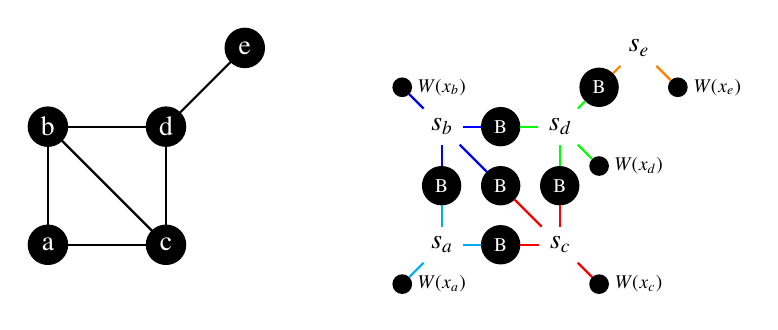
\begin{tikzpicture}[
    dot/.style = {circle, fill, minimum size=#1,
                inner sep=0pt, outer sep=0pt},
    dot/.default = 6pt  % size of the circle diameter 
                    ]  

        \def\dx{0};
        \def\r{0.25cm}
        \filldraw[fill=black] (\dx,0) circle [radius=\r];
        \filldraw[fill=black] (\dx,1.5) circle [radius=\r];
        \filldraw[fill=black] (1.5+\dx,0) circle [radius=\r];
        \filldraw[fill=black] (1.5+\dx,1.5) circle [radius=\r];
        \filldraw[fill=black] (2.5+\dx,2.5) circle [radius=\r];
        \draw [black,thick] (\dx,0) -- (\dx,1.5);
        \draw [black,thick] (\dx,0) -- (1.5+\dx,0);
        \draw [black,thick] (\dx,1.5) -- (1.5+\dx,1.5);
        \draw [black,thick] (1.5+\dx,0) -- (1.5+\dx,1.5);
        \draw [black,thick] (1.5+\dx,0) -- (\dx,1.5);
        \draw [black,thick] (2.5+\dx,2.5) -- (1.5+\dx,1.5);
        \node[color=white] at (\dx,0) {a};
        \node[color=white] at (\dx,1.5) {b};
        \node[color=white] at (1.5+\dx,0) {c};
        \node[color=white] at (1.5+\dx,1.5) {d};
        \node[color=white] at (2.5+\dx,2.5) {e};
        \def\dx{5};
        \def\r{0.25cm}
        \foreach \x/\y/\e in {0.75/0/ac, 0/0.75/ab, 1.5/0.75/cd, 0.75/1.5/bd, 0.75/0.75/bc, 2/2/de}
            \node[color=white,fill=black,dot=2*\r] at (\x+\dx,\y) (\e) {\scriptsize B};
        \foreach \x/\y/\v in {0/0/a, 0/1.5/b, 1.5/0/c, 1.5/1.5/d, 2.5/2.5/e}
            \node[color=black] at (\x+\dx,\y) (\v) {$s_\v$};
        \foreach \x/\y/\v in {-0.5/-0.5/a, -0.5/2.0/b, 2.0/-0.5/c, 2.0/1.0/d, 3.0/2.0/e}
            \node[color=white,fill=black,dot=\r] at (\x+\dx,\y) (\v\v) {};
        \foreach \x/\y/\v in {-0.5/-0.5/a, -0.5/2.0/b, 2.0/-0.5/c, 2.0/1.0/d, 3.0/2.0/e}
            \node[color=black] at (\x+\dx+0.5,\y) {\scriptsize $W(x_\v)$};
        \draw [cyan,thick] (a) -- (aa);
        \draw [cyan,thick] (a) -- (ab);
        \draw [cyan,thick] (a) -- (ac);
        \draw [blue,thick] (b) -- (bb);
        \draw [blue,thick] (b) -- (ab);
        \draw [blue,thick] (b) -- (bc);
        \draw [blue,thick] (b) -- (bd);
        \draw [red,thick] (c) -- (cc);
        \draw [red,thick] (c) -- (ac);
        \draw [red,thick] (c) -- (bc);
        \draw [red,thick] (c) -- (cd);
        \draw [green,thick] (d) -- (dd);
        \draw [green,thick] (d) -- (bd);
        \draw [green,thick] (d) -- (de);
        \draw [green,thick] (d) -- (cd);
        \draw [orange,thick] (e) -- (ee);
        \draw [orange,thick] (e) -- (de);
    \end{tikzpicture}}
    \begin{align*}
        \sum_{s_a,s_b,s_c,s_d,s_e} W(x_a)_{s_a} W(x_b)_{s_b} W(x_c)_{s_c} W(x_d)_{s_d} W(x_e)_{s_e} B_{s_a s_b} B_{s_b s_d} B_{s_a s_c} B_{s_b s_c} B_{s_d s_e}.
    \end{align*}
\end{example}

Before contracting the einsum network and evaluating the independence polynomial numerically, let us first give up thinking $0$s and $1$s in tensors $W(x)$ and $B$ as regular computer numbers such as integers and floating point numbers.
Instead, we treat them as the additive identity and multiplicative identity of a commutative semiring.
A semiring is a ring without additive inverse, while a commutative semiring is a semiring that multiplication commutative.
To define a commutative semiring with addition algebra $\oplus$ and multiplication algebra $\odot$ on a set $R$, the following relation must hold for arbituary three elements $a, b, c \in R$.
\begin{align*}
(a \oplus b) \oplus c = a \oplus (b \oplus c) & \hspace{5em}\text{$\triangleright$ commutative monoid $\oplus$ with identity $\mymathbb{0}$}\\
a \oplus \mymathbb{0} = \mymathbb{0} \oplus a = a &\\
a \oplus b = b \oplus a &\\
&\\
(a \odot b) \odot c = a \odot (b \odot c)  &   \hspace{5em}\text{$\triangleright$ commutative monoid $\odot$ with identity $\mymathbb{1}$}\\
a \odot  \mymathbb{1} =  \mymathbb{1} \odot a = a &\\
a \odot b = b \odot a &\\
&\\
a \odot (b\oplus c) = a\odot b + a\odot c  &  \hspace{5em}\text{$\triangleright$ left and right distributive}\\
(a\oplus b) \odot c = a\odot c \oplus b\odot c &\\
&\\
a \odot \mymathbb{0} = \mymathbb{0} \odot a = \mymathbb{0}
\end{align*}

In the rest of this paper, we show how to obtain the independence polynomial, the maximum independent set size and optimal configurations of a general graph $G$ by designing tensor element types as commutative semirings,
i.e. making the einsum network generic~\cite{Stepanov2014}.

\subsection{The polynomial approach}
A straight forward approach to evaluate the independence polynomial is treating the tensor elements as polynomials, and evaluate the polynomial directly.
Let us create a polynomial type, and represent a polynomial $a_0 + a_1 x + \ldots + a_k x^k$ as a vector $(a_0, a_1, \ldots, a_k) \in R^k$, e.g. $x$ is represented as $(0, 1)$.
We define the algebra between the polynomials $a$ of order $k_a$ and $b$ of order $k_b$ as
\begin{align}
    \begin{split}
    a \oplus b &= (a_0 + b_0, a_1 + b_1, \ldots, a_{\max(k_a, k_b)} + b_{\max(k_a, k_b)}),\\
    a \odot b &= (a_0 + b_0, a_1b_0 + a_0b_1, \ldots, a_{k_a} b_{k_b}),\\
    \mymathbb{0} &= (),\\
    \mymathbb{1} &= (1).\label{eq:polynomial}
    \end{split}
\end{align}
By contracting the einsum network with polynomial type, the final result is the exact representation of the independence polynomial.
In the program, the multiplication can be evaluated efficiently with the convolution theorem.
The only problem of this method is it suffers from a space overhead that propotional to the maximum independant set size because each polynomial requires a vector of such size to store the factors.
In the following subsections, we managed to solve this problem.

\subsection{The fitting and Fourier transformation approaches}
Let $m=\alpha(G)$ be the maximum independent set size and $X$ be a set of $m+1$ random real numbers, e.g. $\{0, 1, 2, \ldots, m\}$.
We compute the einsum contraction for each $x_i \in X$ and obtain the following relations
\begin{align}
    \begin{split}
a_0 + a_1 x_1 + a_1 x_1^2 + \ldots + a_m x_1^m &= y_0\\
a_0 + a_1 x_2 + a_2 x_2^2 + \ldots + a_m x_2^m &= y_1\\
\ldots&\\
a_0 + a_1 x_m + a_2 x_m^2 + \ldots + a_m x_m^m& = y_m
    \end{split}
\end{align}
The polynomial fitting between $X$ and $Y = \{y_0, y_1, \ldots, y_m\}$ gives us the factors.
The polynomial fitting is esentially about solving the following linear equation
\begin{align}
\left(\begin{matrix}
1 & x_1 & x_1^2 & \ldots & x_1^m \\
1 & x_2 & x_2^2 & \ldots & x_2^m \\
\vdots & \vdots & \vdots &\ddots & \vdots \\
1 & x_m & x_m^2 & \ldots & x_m^m
\end{matrix}\right)
\left(\begin{matrix}
a_0 \\ a_1 \\ \vdots \\ a_m
\end{matrix}\right)
= \left(\begin{matrix}
y_0 \\ y_1 \\ \vdots \\ y_m
\end{matrix}\right).\label{eq:lineareq}
\end{align}

In practise, the fitting can suffer from the non-negligible round off errors of floating point operations and produce unreliable results.
This is because the factors of independence polynomial can be different in magnitude by many orders.
Instead of choosing $X$ as a set of random real numbers, we make it form a geometric sequence in the complex domain $x_j = r\omega^j$, where $r \in \mathbb{R}$ and $\omega = e^{-2\pi i/(m+1)}$. The above linear equation becomes
\begin{align}
\left(\begin{matrix}
1 & r\omega & r^2\omega^2 & \ldots & r^m\omega^m \\
1 & r\omega^2 & r^2\omega^4 & \ldots & r^m\omega^{2m} \\
\vdots & \vdots & \vdots &\ddots & \vdots \\
1 & r\omega^m & r^2\omega^{2m} & \ldots & r^m\omega^{m^2}
\end{matrix}\right)
\left(\begin{matrix}
a_0 \\ a_1 \\ \vdots \\ a_m
\end{matrix}\right)
= \left(\begin{matrix}
y_0 \\ y_1 \\ \vdots \\ y_m
\end{matrix}\right).
\end{align}

Let us rearange the factors $r^j$ to $a_j$, the matrix on left side is exactly the a descrete fourier transformation (DFT) matrix.
Then we can obtain the factors using the inverse fourier transformation $\vec a_r = {\rm FFT^{-1}}(\omega) \cdot \vec y$, where $(\vec a_r)_j = a_j r ^j$.
By choosing diferent $r$, one can obtain better precision in low independant set size region  ($\omega<1$) and high independant set size region ($\omega>1$).

\subsection{The finite field algebra approach}
It sounds a bit over ambitious to compute the independence polynomial regorously using integer number types only,
because the fixed width integer types are often too small to store the countings,
while big integer with arbituary precision can be very slow and imcompatible with graphic processing units (GPU) devices.
The solution we found is to computation on a finite field algebra $GF(p)$

\begin{align}
\begin{split}
    x ~\oplus~ y &= x+y\pmod p,\\
    x ~\odot~ y &= xy\pmod p,\\
    \mymathbb{0} &= 0,\\
    \mymathbb{1} &= 1.
\end{split}
\end{align}

In a finite field algebra, we have the following observations
\begin{enumerate}
    \item One can still use Gaussian elimination~\cite{Golub2013} to solve a linear equation \Eq{eq:lineareq}.
    This is because a field has the property that the multiplicative inverse exists for any non-zero value.
    The multiplicative inverse here can be computed with the extended Euclidean algorithm.
    \item Given the remainders of a larger integer $x$ over a set of coprime integers $\{p_1, p_2, \ldots, p_n\}$,
    $x \pmod {p_1 \times p_2 \times \ldots \times p_n}$ can be computed using the chinese remainder theorem.
    With this, one can infer big integers even though its bit width is larger than the register size.
\end{enumerate}
With these observations, we developed Algorithm~\ref{alg:finitefield} to compute independence polynomial exactly without introducing space overheads.
In the algorithm, except the computation of chinese remainder theorem, all computations are done with integers of fixed width $W$.

\begin{algorithm}[!ht]
    \small
    \SetAlgoNoLine
    \LinesNumbered
    Let $P = 1$, vector $X = (0,1,2,\ldots,m)$, matrix $\hat X_{ij} = X_i^j$, where $i,j = 0, 1, \ldots m$\;

    \While{true}{
        compute the largest prime $p$ that $\gcd(p, P) = 1 \land p \leq 2^W$\;

        compute the tensor network contraction on $GF(p)$ and obtain $Y = (y_0, y_1, \ldots , y_m) \pmod p $\;

        $A_p = (a_0, a_1, \ldots, a_m) \pmod p = {\rm gaussian\_elimination}(\hat X, Y \pmod p) $\;

        $A_{P\times p} = {\rm chinese\_remainder}(A_P, A_p)$\;

        \If{$A_P = A_{P \times p}$}{
            \Return $A_P$ \tcp*[l]{converged}
        }
        $P = P \times p$\;
    }\caption{Compute independence polynomial exactly without integer overflow}\label{alg:finitefield}
\end{algorithm}

\section{Computing maximum independent set size and its corresponding degeneracy and configurations}
Obtaining the maximum independent set size and its degeneracy can be computational more efficient. Let $x=\infty$, then the independence polynomial becomes
\begin{equation}
I(G, \infty) = a_k \infty^{\alpha(G)},
\end{equation}
where the lower orders terms disappear automatically. We can define a new algebra as
\begin{align}
\begin{split}
    a_x\infty^x \oplus a_y\infty^y &= \begin{cases}
        (a_x + a_y)\infty^{\max(x,y)}, & x = y\\
        a_y\infty^{\max(x,y)}, & x < y\\
        a_x\infty^{\max(x,y)}, & x > y
    \end{cases}\\
    a_x\infty^x \odot a_y\infty^y &= a_x a_y\infty^{x+y}\\
    \mymathbb{0} &= 0\infty^{-\infty}\\
    \mymathbb{1} &= 1\infty^{0}
\end{split}
\end{align}
In the program, we only store the power $x$ and the corresponding factor $a_x$ that initialized to $1$.
This algebra is consistent with the one we derived in ~\cite{Liu2021} that uses the tropical tensor network for solving spin glass ground states.
If one is only interested in obtaining $\alpha(G)$, he can drop the factor parts, then the algebra of $x$ becomes the max-plus tropical algebra~\cite{Maclagan2015,Moore2011}.

One may also want to obtain all ground state configurations, it can be achieved replacing the factors $a_x$ with a set of bit strings $s_x$.
We design a new element type that having algebra
\iffalse
\begin{align}
\begin{split}
    s_x \oplus s_y &= s_x \cup s_y\\
    s_x \odot s_y &= \{\sigma \lor \tau | \sigma \in s_x, \tau \in s_y\}\\
    \mymathbb{0} &= \{\}\\
    \mymathbb{1} &= \{\boldsymbol 0\}
\end{split}
\end{align}
\fi
\begin{align}
\begin{split}
    s_x\infty^x \oplus s_y\infty^y &= \begin{cases}
        (s_x \cup s_y)\infty^{\max(x,y)}, & x = y\\
        s_y\infty^{\max(x,y)}, & x < y\\
        s_x\infty^{\max(x,y)}, & x > y
    \end{cases},\\
    s_x\infty^x \odot s_y\infty^y &= \{\sigma \lor^\circ \tau | \sigma \in s_x, \tau \in s_y\}\infty^{x+y},\\
    \mymathbb{0} &= \{\}\infty^{-\infty},\\
    \mymathbb{1} &= \{0^{\otimes n}\}\infty^{0},
\end{split}
\end{align}

One can easily check that this replacement does not change the fact that the algebra is a commutative semiring.
We first initialize the bit strings of the variable $x$ in the vertex tensor to a vertex index $i$ dependent onehot vector $x_i = \boldsymbol{e}_{i}$,
then we contract the tensor network. The resulting object will give us the set of all optimal configurations.
By slightly modifying the above algebra, it can also be used to obtain just a single configuration to save computational effort.
%We leave this as an exercise for readers.

\begin{align}
\begin{split}
    \sigma_x\infty^x \oplus \sigma_y\infty^y &= \begin{cases}
        {\rm select}(\sigma_x, \sigma_y)\infty^{\max(x,y)}, & x = y\\
        \sigma_y\infty^{\max(x,y)}, & x < y\\
        \sigma_x\infty^{\max(x,y)}, & x > y
    \end{cases},\\
    \sigma_x\infty^x \odot \sigma_y\infty^y &= (\sigma_x \lor^\circ \sigma_y)\infty^{x+y},\\
    \mymathbb{0} &= 1^{\otimes n}\infty^{-\infty},\\
    \mymathbb{1} &= 0^{\otimes n}\infty^{0},
\end{split}
\end{align}
where the \texttt{select} function picks one of $\sigma_x$ and $\sigma_y$.
One can decide an order by some criteria to make the algebra commutative and associative.
In most cases, it does not matter if one pick randomly from them, the program just output one of optimal configuration randomly.

\subsection{counting sub-optimal solutions}
Some times people are interested in finding sub-optimal solutions efficiently.
We modify the polynomial algebra a bit by keeping only largest two factors in the polynomial in \Eq{eq:polynomial}.
\begin{align}
    \begin{split}
    a \oplus b &= (a_{\max(k_a, k_b)-1} + b_{\max(k_a, k_b)-1}, a_{\max(k_a, k_b)} + b_{\max(k_a, k_b)}),\\
    a \odot b &= (a_{k_a-1} b_{k_b}+a_{k_a} b_{k_b-1}, a_{k_a} b_{k_b}),\\
    \mymathbb{0} &= (),\\
    \mymathbb{1} &= (1).\label{eq:polynomial}
    \end{split}
\end{align}
By changing the factors to sets, and plus and multiplication operations on factors to set union and product, one can get all suboptimal solutions too.

\subsection{bounding the enumeration space}
When we try to implement the above algebra for enumerating configurations, we find the space overhead is larger than than we have expected.
It stores more than nessesary intermedite configurations. To speed up the computation, we use $\alpha(G)$ that much easier to compute for bounding.
We first compute the value of $\alpha(G)$ with tropical numbers and cache all intermediate tensors.
Then we compute a boolean masks for each cached tensor, where we use a boolean true to represent a tensor element having contribution to the maximum independent set (i.e. with a nonzero gradient) and boolean false otherwise.
Finally, we perform masked matrix multiplication using the new element type with the above algebra for obtaining all configurations.
To compute the masks, we ``back propagate'' the masks step by step through contraction process using the cached intermediate tensors.
Consider a tropical matrix multiplication $C = A B$, we have the following inequality
\begin{align}
    A_{ij} \odot B_{jk} &\leq C_{ik}.
\end{align}

Moving $B_{ik}$ to the right hand side, we have
\begin{align}
    A_{ij} &\leq (\oplus_{k} (C_{ik}^{-1} \odot B_{jk}))^{-1}
\end{align}
where the tropical multiplicative inverse is defined as the additive inverse of the regular algebra. The equality holds if and only if element $A_{ij}$ contributions to $C$ (i.e. has nonzero gradient).
Let the mask for $C$ being $\overline C$, the backward rule for gradient masks reads
\begin{align}
\overline{A}_{ij} = \delta(A_{ij}, ((C^{\circ-1} \circ \overline C )B^T)_{ij}^{\circ -1}),
\end{align}
where ${}^{\circ -1}$ is the Hadamard inverse, $\circ$ is the Hadamard product, boolean false is treated as tropical zero and boolean true is treated as tropical one.
This rule defined on matrix multiplication can be easily generalized to the einsum of two tensors by replacing the matrix multiplication between $C^{\circ-1} \circ \overline C$ and $B^T$ by an einsum.

\section{Counting maximal independent sets}
Let us denote the neighbor of a vertex $v$ as $N(v)$ and $N[v] = N(v)\cup \{v\}$.
A maximal independent set $I_m$ is an independent sets that there is no such vertex $v$ that $N[v] \cap I_m = \emptyset$.
Let us modify the einsum network for computing independence polynomial to count maximal independent sets.
We define a tensor on $N[v]$ to capture this property
\begin{align}
    T(x)_{s_1,s_2,\ldots,s_{|N(v)|},s_v} = \begin{cases}
        s_vx & s_1=s_2=\ldots=s_{|N(v)|}=0,\\
        1-s_v& otherwise.\\
    \end{cases}
\end{align}
As an example, for a vertex of degree 2, the resulting rank 3 tensor is
\begin{align}
    T(x)=\left(\begin{matrix}
    \left(\begin{matrix}
        0 &1 \\
        1 &1
    \end{matrix}\right)\\
    \left(\begin{matrix}
        x &0 \\
        0 &0
    \end{matrix}\right)
    \end{matrix}\right).
\end{align}

We do the same computation as independence polynomial, the coefficients of resulting polynomial gives the counting of maximal independent sets.
In many sparse graphs, this tensor network contraction approach is much faster than computing the maximal cliques of its complement and use Bron Kerbosch algorithms for finding maximum cliques.
However, the treewidth of this new tensor network is larger than the one for independence polynomial because it can not utilize some structures of the original graph,
while the original tensor network can be trivially reduced to this one.
We will use an example in the appendix to show why this tensor network is harder to contract.

\section{Automated branching}
% check http://www.tcs.rwth-aachen.de/independentset/ for more rules
Branching rules can be automatically discovered by contracting the tropical einsum network for a subgraph $R \subseteq G$.
Let us denote the resulting tropical tensor of rank $|C|$ as $A$, where $C$ is the set of boundary vertices defined as $C := \{c | c\in R \land c \in G\backslash R\}$ and $|C|$ the size of $C$.
Each tensor entry $A_{\sigma}$ is a local maximum independant set size with a fixed boundary configuration $\sigma \in \{0,1\}^{|C|}$ by marginalizing the inner degrees of freedom.
If we are only interested in finding a single maximum independent set rather than enumerating all possible solutions,
this tensor can be further ``compresed'' by setting some entries to tropical zero.
Let us define a relation of \textit{less restrictive} as
\begin{align}
(\sigma_a \prec \sigma_b) := (\sigma_a \neq \sigma_b) \land (\sigma_a \leq^\circ \sigma_b)
\end{align}
where $\leq^\circ$ is the Hadamard less or equal operations.

\begin{definition}
A tensors $A$ is \textit{MIS-compact} if are no two nonzero entries of it that one is ``better'' than another,
where an entry $A_{\sigma_a}$ is ``better'' than $A_{\sigma_b}$ if
\begin{align}
(\sigma_a \prec \sigma_b) \land (A_{\sigma_a} \geq A_{\sigma_b})\label{eq:compress}.
\end{align}
\end{definition}

If we remove such $A_{\sigma_b}$, the contraction over the whole graph is guaranted to give the same maximum independant set size.
It can be seen by considering two entries with the same local maximum independent set sizes and different boundary configurations as shown in \Fig{fig:compressrule} (a) and (b).
If we have $\sigma_b \cup \overline{\sigma_b}$ being one of the solutions for maximum independant sets in $G$, then $\sigma_a \cup \overline{\sigma_b}$ is another solution giving the same $\alpha(G)$.
Hence, we can set $A_{\sigma_b}$ to tropical zero safely.
%among boundary configurations with equal local maximum independent sizes,
%we only retain those least restrictive (less ones at the boundary) to exterial configurations.

\begin{figure}
    \centering
    \includegraphics[width=0.8\textwidth, trim={5cm 4cm 5cm 4cm}, clip]{compressionrule.pdf}
    \caption{Two configurations with the same local independent size $A_{\sigma_a} = A_{\sigma_b} = 3$ and different boundary configurations (a) $\sigma_a=\{001\}$ and (b) $\sigma_b = \{101\}$, where black nodes are $1$s (in the independent set) and white nodes are $0$s (not in the independent set).}\label{fig:compressrule}
\end{figure}

\begin{theorem}[]
    A MIS-compact tropical tensor is optimal, i.e. none of its none zero entries can be removed without accessing global information.
\end{theorem}

\begin{proof}
    %Given $A_\{\sigma_a}$ is better than $A_\{\sigma_b\}$, any exterior configuration $\overline{\sigma}$ making $\overline{\sigma} \cup \sigma_b$ a global maximum independent set also makes $\overline{\sigma} \cup \sigma_a$ a maximum independent set.
    Let use prove it by showing $\forall \sigma$ in a MIS-compact tropical tensor for a subgraph $R$, there exists a graph $G$ that $R\subseteq G$ and $\sigma$ is the only boundary configuration that produces the maximum independent set.
    i.e. no tensor entry can be removed without knowledge about $G\backslash R$.
    Let $A$ be a tropical tensor, and an entry of it being $A_{\sigma}$, where $\sigma$ is the bounary configuration.
    Let us construct a graph $G$ such that for a vertex $v \in C$, if $\sigma_v=1$, $\alpha(N[v] \cap (G \backslash R)) = 0$, otherwise, $\alpha(N[v] \cap (G\backslash R)) = \infty$, meanwhile, for any $v, w \in C$, $N[v]\cap N[w] = \emptyset$.
    The simplest construction is connecting vertices that $\sigma_v=0$ with infinite many mutually disconnected vertices as illustrated in the following graph.

    \centerline{\includegraphics[width=0.35\textwidth, trim={0cm 2cm 6cm 0cm}, clip]{proofoptimal.pdf}}

    Then we have the maximum independent set size with boundary configuration $\sigma$ being $\alpha(G,\sigma) = \infty (|C|-|\sigma|) + A_{\sigma}$,
    where $|\sigma|$ is defined as the number of $1$s in $\sigma$.
    Let us assume there exists another configuration $\tau$ that generating the same or even better maximum independent set size $\alpha(G, \tau) \geq \alpha(G, \sigma)$.
    Then we have $\tau \prec \sigma$, otherwise it will suffer from infinite punishment from $G\backslash R$.
    For such a $\tau$, we have $A_\tau < A_\sigma$, otherwise $A_\sigma \prec A_\tau$ contradicts with $A$ being MIS-compact.
    Finally, we have $\alpha(G,\tau) = \infty (|C|-|\sigma|) + A_{\tau} < \alpha(G,\sigma)$, which contradicts with our preassumtion. Such $\tau$ does not exist and $\sigma$ is the only boundary configuration that $\alpha(G) = \alpha(G, \sigma)$.
\end{proof}

\subsection{The tensor network compression detects branching rules automatically}
In the following, we are going to show tropical tensor networks with least restrictive principle can automatically discover branching rules.
We denote the effective branching number of contracting the local degrees of freedoms as $\left|\{A_{\sigma} \neq \mymathbb{0}\right|\sigma \in \{0, 1\}^{|C|}\}|/2^{|R|}$.
It is the effective degree of freedoms per vertex in $R$.

\begin{corollary}\label{rule:one} % basic
  If a vertex $v$ is in an independent set $I$, then none of its neighbors can be in $I$.
On the other hand, if $I$ is a maximum (and thus maximal) independent set,
and thus if $v$ is not in $I$ then at least one of its neighbors is in $I$.
\end{corollary}

Contract $N[v]$ and the resulting tensor $A$ has a rank $|N(v)|$. Each tensor entry $A_{\sigma}$ corresponds to a locally maximized independant set size with fixed boundary configuration $\sigma \in \{0, 1\}^{|N(v)|}$.
If the boundary configuration is a bit string of 0s, $\sigma_v$ will takes value $1$ to maximize the local independant set size.

\centerline{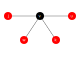
\includegraphics[width=0.4\columnwidth,trim={0 3.5cm 0 1cm},clip]{../notebooks/basic.pdf}}

After contracting $N[v]$, $v$ becomes an internal degree of freedom.
Applying tensor compression rule \Eq{eq:compress}, the resulting rank 4 tropical tensor is

\begin{align}
    T_{juwk} = \left(\begin{matrix}
        \left(\begin{matrix}
        ~~~~1 & -\infty \\
        -\infty & ~~~~2
        \end{matrix}\right)_{ju}&
        \left(\begin{matrix}
        -\infty & ~~~~2 \\
        ~~~~2 & ~~~~3
        \end{matrix}\right)_{ju}\\
        \left(\begin{matrix}
        -\infty & ~~~~2 \\
        ~~~~2 & ~~~~3
        \end{matrix}\right)_{ju} &
        \left(\begin{matrix}
        ~~~~2 & ~~~~3 \\
        ~~~~3 & ~~~~4
        \end{matrix}\right)_{ju}
    \end{matrix}\right)_{wk}.
\end{align}

The effective branching value is $11^{1/5} \approx 1.6154$, which is larger than the branching number $\tau(1, 5) \approx 1.3247$.
It does not mean the tropical tensor does not find all the branches, if we contract $N^2[v]$.

\begin{corollary}[mirror rule] % 2.7
For some $v \in V$, a node $u \in N^2(v)$ is called mirror of $v$, if $N(v) \backslash N(u)$ is a clique. We denote the set of of a node $v$ mirrors~\cite{Fomin2013} by $M(v)$.
Let $G = (V, E)$ be a graph and $v$ a vertex of $G$. Then
\begin{equation}
\alpha(G) = \max(1 + \alpha(G \backslash N[v]), \alpha(G \backslash (M(v) \cup \{v\})).
\end{equation}
\end{corollary}

This rule states that if $v$ is not in $M$, there exists an MIS $I$ that $M(v)\notin I$.
otherwise, there must be one of $N(v)$ in the MIS (\textit{local maximum rule}).
If $w$ is in $I$, then none of $N(v) \cap N(w)$ is in $I$, then there must be one of node in the clique $N(v)\backslash N(w)$ in $I$ (\textit{local maximum rule}),
since clique has at most one node in the MIS, by moving the occuppied node to the interior, we obtain a ``better'' solution.
%Hence, the \textit{least restrictive principle} captures the mirror rule.

In the following example, since $u\in N^2(v)$ and $N(v) \backslash N(u)$ is a clique, $u$ is a mirror of $v$.

\centerline{\includegraphics[width=0.4\columnwidth,trim={0 3.5cm 0 1cm},clip]{../notebooks/mirror.pdf}}

After contracting $N[v]\cup u$, $v$ becomes an internal degree of freedom.
Applying tensor compression rule \Eq{eq:compress}, the resulting rank 4 tropical tensor is

\begin{align}
    T_{juwk} = \left(\begin{matrix}
        \left(\begin{matrix}
        ~~~~1 & ~~~~2 \\
        -\infty & -\infty
        \end{matrix}\right)_{ju}&
        \left(\begin{matrix}
        -\infty & -\infty \\
        ~~~~2 & -\infty
        \end{matrix}\right)_{ju}\\
        \left(\begin{matrix}
        -\infty & -\infty \\
        -\infty & -\infty
        \end{matrix}\right)_{ju} &
        \left(\begin{matrix}
        -\infty & -\infty \\
        -\infty & -\infty
        \end{matrix}\right)_{ju}
    \end{matrix}\right)_{wk}.
\end{align}

In this case, the effective branching number is $3^{1/5}\approx 1.2457$,
which is smaller than the branching number $\tau(4, 2) = 1.2721$ by simply applying the mirror rule.

\begin{corollary}[satellite rule] % satellite rule
Let $G$ be agraph $v \in V$. A node $u \in N^2(v)$ is called satellite~\cite{Kneis2009} of $v$, if there is some $u' \in N(v)$ such that $N[u'] \backslash N[v] = \{u\}$.
The set of satellites of a node $v$ is denotedby $S(v)$, and we also use the notation $S[v] := S(v) \cup {v}$. Then 
\begin{equation}
\alpha(G) = \max\{\alpha(G \backslash \{v\}), \alpha(G \backslash N[S[v]]) + |S(v)| + 1\}.
\end{equation}
\end{corollary}

This rule can be capture by contracting $N[v] \cup S(v)$.
In the following example, since $u \in N^2(v)$ and $w \in N(v)$ satisfies $N[w] \backslash N[v] = \{u\}$, $u$ is a satellite of $v$.

\centerline{\includegraphics[width=0.4\columnwidth,trim={0 3.5cm 0 1cm},clip]{../notebooks/satellite.pdf}}

After contracting $N[v] \cup u$, both $v$ and $w$ become internal degrees of freedoms.
Applying tensor compression rule \Eq{eq:compress}, the resulting rank 3 tropical tensor is
\begin{align}
    T_{juk} = \left(\begin{matrix}
        \left(\begin{matrix}
        ~~~~1 & ~~~~2 \\
        ~~~~2 & -\infty
        \end{matrix}\right)_{ju}\\
        \left(\begin{matrix}
        -\infty & -\infty \\
        -\infty & -\infty
        \end{matrix}\right)_{ju}
    \end{matrix}\right)_{k}.
\end{align}

There are 3 nonzero entries. The internal configurations of entry $T(j=1, u=0, k=0) = 2$ is $(v=0, w =1)$,
that of entry $T(j=0, u=1, k=0)=2$ is $(v=1, w=0)$, and that of entry $T(j=0, u=0, k=0)=1$ is $(v=1, w=0)$ or $(v=0, w=1)$.
For entry $T(j=0, u=0, k=0)=1$, we post-select the internal degree of freedom as $(v=0, w=1)$.
Then we can see the satellite rule either ${v, u} \in I$ or $v \notin I$ is satisfied.
In this case, the effective branching number is $3^{1/5}\approx 1.2457$. 

\subsection{gadget design}

Suppose we have a local structure as the following.

\centerline{\begin{tikzpicture}[scale=1.0]
    \def\r{0.2}
    \foreach \x/\y [count=\i] in {0.17/0.5,0.83/0.5,0.5/0.67,0.5/0.33}
        \node[fill=red,circle,radius=\r] at (\x*8, \y*8) (\i) {};
    \draw (1) -- (2);
    \draw (3) -- (4);
\end{tikzpicture}}


Contract this local structure gives the tropical tensor

\begin{align}
    \left(\begin{matrix}
        \left(\begin{matrix}
            ~~~~0 & ~~~~1\\
            ~~~~1 & ~~~~2
        \end{matrix}\right) &
        \left(\begin{matrix}
            ~~~~1 & -\infty\\
            ~~~~2 & -\infty
        \end{matrix}\right) \\
        \left(\begin{matrix}
            ~~~~1 & ~~~~2\\
            -\infty & -\infty
        \end{matrix}\right) &
        \left(\begin{matrix}
            ~~~~2 & -\infty\\
            -\infty & -\infty
        \end{matrix}\right)
    \end{matrix}\right).
\end{align}

The following gadget is equivalent to the above diagram up to a constant $2$.

\centerline{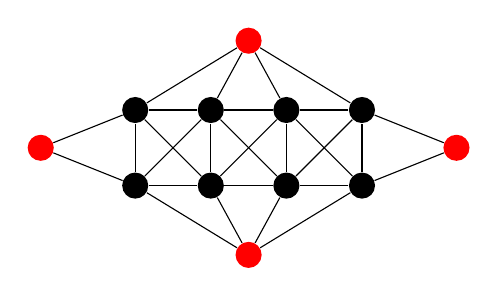
\begin{tikzpicture}
    \def\nodes{(0.5, 0.33), (0.17, 0.5), (0.5, 0.67), (0.83, 0.5), (0.32, 0.44), (0.44, 0.44), (0.56, 0.44), (0.68, 0.44), (0.32, 0.56), (0.44, 0.56), (0.56, 0.56), (0.68, 0.56)}
    \def\edges{(1, 5), (1, 6), (1, 7), (1, 8), (2, 5), (2, 9), (3, 9), (3, 10), (3, 11), (3, 12), (4, 8), (4, 12), (5, 6), (5, 9), (5, 10), (6, 7), (6, 9), (6, 10), (6, 11), (7, 8), (7, 10), (7, 11), (7, 12), (8, 11), (8, 12), (9, 10), (10, 11), (11, 12)}
    \def\r{0.2}
    \foreach \p [count=\i] in \nodes{
        \parsept{\x}{\y}{\p}
        \pgfmathparse{((\x<0.2 || \x>0.8 || \y<0.35 || \y>0.65) ? 1 : 0)}
        \ifnum\pgfmathresult>0
            \node[fill=red,circle,radius=\r] at (\x*8, \y*8) (\i) {};
        \else
            \node[fill,circle,radius=\r] at (\x*8, \y*8) (\i) {};
        \fi
    }
    \foreach \e [count=\i] in \edges{
        \parsept{\x}{\y}{\e}
        \draw (\x) -- (\y);
    }
\end{tikzpicture}}

\begin{align}
    \left(\begin{matrix}
        \left(\begin{matrix}
            ~~~~2 & ~~~~3\\
            ~~~~3 & ~~~~4
        \end{matrix}\right) &
        \left(\begin{matrix}
            ~~~~3 & ~~~~3\\
            ~~~~4 & ~~~~4
        \end{matrix}\right) \\
        \left(\begin{matrix}
            ~~~~3 & ~~~~4\\
            ~~~~2 & ~~~~3
        \end{matrix}\right) &
        \left(\begin{matrix}
            ~~~~4 & ~~~~4\\
            ~~~~3 & ~~~~4
        \end{matrix}\right)
    \end{matrix}\right)
    \xrightarrow[\text{compress, -2}]{}
    \left(\begin{matrix}
        \left(\begin{matrix}
            ~~~~0 & ~~~~1\\
            ~~~~1 & ~~~~2
        \end{matrix}\right) &
        \left(\begin{matrix}
            ~~~~1 & -\infty\\
            ~~~~2 & -\infty
        \end{matrix}\right) \\
        \left(\begin{matrix}
            ~~~~1 & ~~~~2\\
            -\infty & -\infty
        \end{matrix}\right) &
        \left(\begin{matrix}
            ~~~~2 & -\infty\\
            -\infty & -\infty
        \end{matrix}\right)
    \end{matrix}\right)
\end{align}

We can see these two subgraphs produce exactly the same tensors.

\section{benchmarks}
We run a sequetial program benchmark on CPU Intel(R) Core(TM) i5-10400 CPU @ 2.90GHz, and show the results bellow.
\begin{figure}
    \centering
    \includegraphics[width=0.8\textwidth, trim={0cm 0cm 0cm 0cm}, clip]{benchmark.pdf}
    \caption{Benchmark results for computing different properties with different element types.
    }\label{fig:benchmark}
\end{figure}
Einsum network contraction is parallelizable. When the element type is immutable, one can just upload the data to GPU to enjoy the speed up.

\section{discussion}
We introduced in the main text how to compute the indenpendence polynomial, maximum independent set and optimal configurations.
It is interesting that although these properties are global,
they can be solved by designing different element types that having two operations $\oplus$ and $\odot$ and two special elements $\mymathbb{0}$ and $\mymathbb{1}$.
One thing in common is that they all defines a commutative semiring.
Here, we want the $\oplus$ and $\odot$ operations being commutative because we do not want the contraction result of an einsum network to be sensitive to the contraction order.
We show most of the implementation in Appendix \ref{sec:technical}. It is supprisingly short.
The style that we program is called generic programming,
it is about writing a single copy of code, feeding different types into it, and the program computing the result with a proper performance.
It is language dependent feature. If someone want to implement this algorithm in python,
one has to rewrite the matrix multiplication for different element types in C and then export the interface to python.
In C++, users can use templates for such a purpose.
In our work, we chose Julia because its just in time compiling is very powerful that it can generate fast code dynamically for users.
Elements of fixed size, such as the finite field algebra, tropical number, tropical number with counting/configuration field used in the main text can be inlined in an array.
Furthermore, these inlined arrays can be upload to GPU devices for faster generic matrix multiplication implemented in CUDA.jl.

\begin{table}[h!]\centering
\begin{minipage}{0.9\columnwidth}
\ra{1.3}
    \scalebox{1.0}{
        \begin{tabularx}{\textwidth}{bb}\toprule
            \hline
            \textbf{element type}     & \textbf{purpose} \\
            {regular number}     & {counting all indenepent sets} \\
            {tropical number}     & {finding the maximum independent set size} \\
            {tropical number with counting}     & {finding both the maximum independent set size and its degeneracy} \\
            {tropical number with configuration}     & {finding the maximum independent set size and one of the optimal configurations} \\
            {tropical number with multiple configurations}     & {finding the maximum independent set size and all optimal configurations} \\
            {polynomial}     & {computing the indenpendence polynomials exactly} \\
            {complex number}     & {fitting the indenpendence polynomials with fast fourier transformation} \\
            {finite field algebra}     & {fitting the indenpendence polynomials exactly using number theory} \\
            \bottomrule
        \end{tabularx}
    }
    \caption{Tensor element types used in the main text and their purposes.}\label{tbl:generictypes}
\end{minipage}
\end{table}


\bibliographystyle{siamplain}
\bibliography{refs}

\appendix

\section{Technical guide}\label{sec:technical}
\begin{description}
	\item[OMEinsum] a package for einsum,
	\item[OMEinsumContractionOrders] a package for finding the optimal contraction order for einsum \\ \href{https://github.com/Happy-Diode/OMEinsumContractionOrders.jl}{https://github.com/Happy-Diode/OMEinsumContractionOrders.jl},
	\item[TropicalGEMM] a package for efficient tropical matrix multiplication (compatible with OMEinsum),
	\item[TropicalNumbers] a package providing tropical number types and tropical algebra, one o the dependency of TropicalGEMM,
	\item[LightGraphs] a package providing graph utilities, like random regular graph generator,
	\item[Polynomials] a package providing polynomial algebra and polynomial fitting,
	\item[Mods and Primes] packages providing finite field algebra and prime number generators.
\end{description}

One can install these packages by opening a julia REPL, type \colorbox{lightgray}{\texttt{]}} to enter the \texttt{pkg>} mode and type, e.g.
\begin{lstlisting}
pkg> add OMEinsum LightGraphs Mods Primes FFTW Polynomials TropicalNumbers
\end{lstlisting}

It may supprise you that the Julia implementation of algorithms introduced in the paper is so short that except the bounding and sparsity related parts,
all are contained in this appendix. After installing required packages, one can open a Julia REPL and copy the following code into it.

\lstinputlisting[breaklines]{../democode/demo.jl}

In the above examples, the configuration enumeration is very slow, one should use the optimal MIS size for bounding as decribed in the main text.
We will not show any example about implementing the backward rule here because it has approximately 100 lines of code.
Please checkout our Github repository \href{https://github.com/Happy-Diode/NoteOnTropicalMIS}{https://github.com/Happy-Diode/NoteOnTropicalMIS}.

\section{When tensor network is worse than einsum network}\label{app:tensorbad}

Given a graph

\centerline{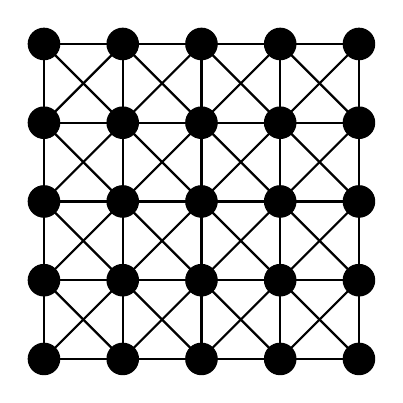
\begin{tikzpicture}
    \def\r{0.2}
    \foreach \x in {1,...,5}
        \foreach \y in {1,...,5}
            \filldraw[fill=black] (\x,\y) circle [radius=\r];
    \foreach \x in {1,...,5}
        \foreach \y in {1,...,4}{
            \draw [black,thick] (\x,\y) -- (\x,\y+1);
            \draw [black,thick] (\y,\x) -- (\y+1,\x);
        }
    \foreach \x in {1,...,4}
        \foreach \y in {1,...,4}{
            \draw [black,thick] (\x,\y) -- (\x+1,\y+1);
            \draw [black,thick] (\y+1,\x) -- (\y,\x+1);
        }
\end{tikzpicture}}

Its tensor network representation is

\centerline{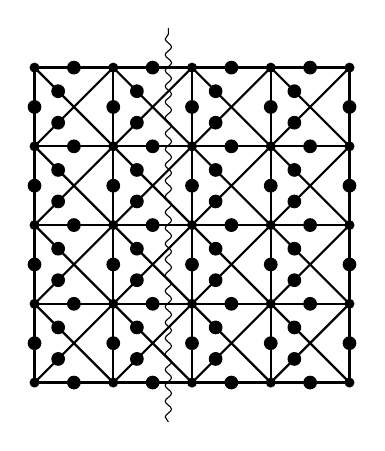
\begin{tikzpicture}
    \def\r{0.08}
    \def\a{0.1}
    \foreach \x in {1,...,5}
        \foreach \y in {1,...,5}
            \filldraw[fill=black] (\x,\y) circle [radius=0.7*\r];
    \foreach \x in {1,...,5}
        \foreach \y in {1,...,4}{
            \filldraw[fill=black] (\x,\y+0.5) circle [radius=\r];
            \filldraw[fill=black] (\y+0.5,\x) circle [radius=\r];
            \draw [black,thick] (\x,\y) -- (\x,\y+1);
            \draw [black,thick] (\y,\x) -- (\y+1,\x);
        }
    \foreach \x in {1,...,4}
        \foreach \y in {1,...,4}{
            \filldraw[fill=black] (\x+0.3,\y+0.3) circle [radius=\r];
            \filldraw[fill=black] (\y+0.3,\x+0.7) circle [radius=\r];
            \draw [black,thick] (\x,\y) -- (\x+1,\y+1);
            \draw [black,thick] (\y+1,\x) -- (\y,\x+1);
        }
    \tikzset{decoration={snake,amplitude=.4mm,segment length=2mm,
                    post length=0mm,pre length=0mm}}
    \draw [decorate] (2.7, 0.5) -- (2.7, 5.5);
\end{tikzpicture}}

Once we represent a $\delta$ tensor as a general tensor, the complexity of this contraction is $\approx 2^{2L}$.
Its einsum network representation is

\centerline{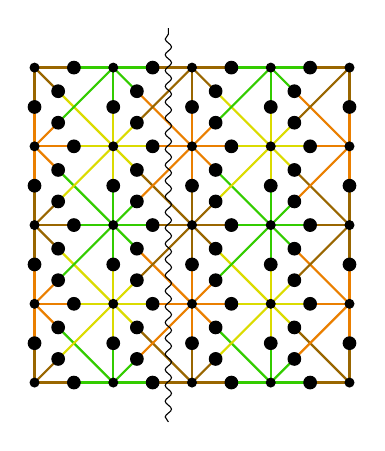
\begin{tikzpicture}
    \def\r{0.08}
    \def\a{0.07}
    \def\L{0.6}
    \def\l{0.1}
    \def\sql{0.24}
    \foreach[evaluate={\cr=0.1+0.5*Mod(\x,2)}] \x in {1,...,5}
        \foreach[evaluate={\cg=0.1+0.3*Mod(\y,2); \cy=0.5-0.5*Mod(\y,2)}] \y in {1,...,5}{
            %\filldraw [red, opacity=0.3] plot [smooth cycle] coordinates {(\x-\L,\y+\l) (\x-\l*2.5,\y+\l) (\x-\L*0.75,\y+\L*0.6) (\x-\L*0.6,\y+\L*0.75) (\x-\l,\y+\l*2.5) (\x-\l, \y+\L) (\x+\l,\y+\L) (\x+\l,\y+\l*2.5) (\x+\L*0.6,\y+\L*0.75) (\x+\L*0.75,\y+\L*0.6) (\x+\l*2.5,\y+\l) (\x+\L,\y+\l) (\x+\L,\y-\l) (\x+\l,\y-\l) (\x+\l,\y-\L) (\x-\l,\y-\L) (\x-\l,\y-\l) (\x-\L,\y-\l)};
            \ifnum \x < 5
                \draw [thick, color={rgb:red,\cr;green,\cg;yellow,\cy}, opacity=1.0, line cap=round] (\x,\y) -- (\x+0.5,\y);
                \ifnum \y < 5
                \draw [thick, color={rgb:red,\cr;green,\cg;yellow,\cy}, opacity=1.0, line cap=round] (\x,\y) -- (\x+0.3,\y+0.3);
                \fi
                \ifnum \y > 1
                \draw [thick, color={rgb:red,\cr;green,\cg;yellow,\cy}, opacity=1.0, line cap=round] (\x,\y) -- (\x+0.3,\y-0.3);
                \fi
            \fi
            \ifnum \x > 1
                \draw [thick, color={rgb:red,\cr;green,\cg;yellow,\cy}, opacity=1.0, line cap=round] (\x,\y) -- (\x-0.5,\y);
                \ifnum \y < 5
                \draw [thick, color={rgb:red,\cr;green,\cg;yellow,\cy}, opacity=1.0, line cap=round] (\x,\y) -- (\x-0.7,\y+0.7);
                \fi
                \ifnum \y > 1
                \draw [thick, color={rgb:red,\cr;green,\cg;yellow,\cy}, opacity=1.0, line cap=round] (\x,\y) -- (\x-0.7,\y-0.7);
                \fi
            \fi
            \ifnum \y < 5
                \draw [thick, color={rgb:red,\cr;green,\cg;yellow,\cy}, opacity=1.0, line cap=round] (\x,\y) -- (\x,\y+0.5);
            \fi
            \ifnum \y > 1
                \draw [thick, color={rgb:red,\cr;green,\cg;yellow,\cy}, opacity=1.0, line cap=round] (\x,\y) -- (\x,\y-0.5);
            \fi
        }
    \foreach \x in {1,...,5}
        \foreach \y in {1,...,5}{
            \filldraw[fill=black] (\x,\y) circle [radius=0.7*\r];
        }
    \foreach \x in {1,...,5}
        \foreach \y in {1,...,5}{
            \ifnum \y < 5
                \filldraw[fill=black] (\x,\y+0.5) circle [radius=\r];
                \filldraw[fill=black] (\y+0.5,\x) circle [radius=\r];
            \fi
        }
    \foreach \x in {1,...,4}
        \foreach \y in {1,...,4}{
            \filldraw[fill=black] (\x+0.3,\y+0.3) circle [radius=\r];
            \filldraw[fill=black] (\y+0.3,\x+0.7) circle [radius=\r];
        }
    \tikzset{decoration={snake,amplitude=.4mm,segment length=2mm,
                    post length=0mm,pre length=0mm}}
    \draw [decorate] (2.7, 0.5) -- (2.7, 5.5);
\end{tikzpicture}}

\section{Generalizing to other graph problems}
Courcelle’s theorem~\cite{Courcelle1990,Barr2020} states that a problem quantified by monadic second order logic (MSO) on a graph with bounded treewidth $k$ can be solved in linear time with respect to the graph size.
Dynamic programming is a traditional approach to attack a $MSO$ problem, it can solve the MIS problem in $O(2^k)n$.
An einsum network is closely related to dynamic programming.
To be specific, the contraction of a einsum network is a special type of dynamic programming that its update rule can be characterized by a linear operation.
An einsum network is strictly less expressive than $MSO$, the einsum network described by \Eq{eq:wtensor} and \Eq{eq:btensor} can be expressed in MSO as
\begin{align}
    \begin{split}
    \exists_X\forall_{u} (\forall_{v} {\rm adj}(u, v) \land (
        &(u \not\in X \land v \not\in X \land B_{00}) \lor\\
        &(u \not\in X \land v \in X \land B_{01}) \lor\\
        &(u \in X \land v \not\in X \land B_{10}) \lor\\
        &(u \in X \land v \in X \land B_{11})
    ))\land\\
    (
        &(u \not\in X \land W_{0}) \lor\\
        &(u \in X \land W_{1})
    ),
    \end{split}
\end{align}
while not all monadic second order logic can be represented as an einsum network contraction,
for example, it is hard to construct a tensor network to decide whether a graph is connected or not.
At the cost of lossing expressiveness, we can encode the properties of the graph into the tensor elements.

In the following, we introduce several other problems that can be solved in the framework of generic einsum network in $O(2^k n)$.
The first one is the matching polynomials.
A match polynomial of a graph $G$ is defined as
\begin{align}
    M(G, x) = \sum\limits_{k=1}^{|V|/2} c_k x^k,
\end{align}
where $k$ is the number of matches, and coefficients $c_k$ are countings.

We define a tensor of rank $d(v) = |N(v)|$ on vertex $v$ such that,
\begin{align}
    W_{v\rightarrow n_1, v\rightarrow n_2, \ldots, v\rightarrow n_{d(v)}} = \begin{cases}
        1, & \sum_{i=1}^{d(v)} v\rightarrow n_i \leq 1,\\
        0, & otherwise,
    \end{cases}
\end{align}
and a tensor of rank $1$ on the bond
\begin{align}
    B_{v\rightarrow w} = \begin{cases}
    1, & v \rightarrow w = 0 \\
    x, & v \rightarrow w = 1.
\end{cases}
\end{align}

Here, we use bond index $v \rightarrow w$ to label tensors.

\end{document}
